\documentclass[a4paper, 11pt]{article}
\usepackage[utf8]{inputenc} 
\usepackage[T1]{fontenc}
\usepackage{lmodern}
\usepackage[french]{babel}
\usepackage{hyperref}

\usepackage{amsmath}
\usepackage{amssymb}
\usepackage{amsthm}
\usepackage{mathtools}
\usepackage{listings}

\usepackage{graphicx}
\usepackage{tikz}
\usetikzlibrary{calc,trees,positioning,arrows,chains,shapes.geometric,%
    decorations.pathreplacing,decorations.pathmorphing,shapes,%
    matrix,shapes.symbols,fit,arrows.meta,backgrounds}

\usepackage{pgfplots} 

\theoremstyle{definition}
\newtheorem{definition}{Definition}[section]

\graphicspath{ {./images/} }


\begin{document}

\title{Étude de joueur artificiel de jeu de grande stratégie}
\author{Dimitri \bsc{Cocheril-Crèvecœur}}
\date{2023-2024}

\maketitle

\section*{Introduction}
J'étudie un modèle de joueur artificiel de jeu de grande stratégie (aussi appelé RTS).
Les RTS sont un genre de jeu de stratégie, sans meilleure stratégie, en temps réel, avec un grand espace d'action.
J'ai décidé de travailler principalement sur l'adaptation de l'application du Monte Carlo Tree Search (MCTS) au problème.


\section*{Présentation}
On pose les contraintes auxquelles on va répondre :\\
On travaille sur les IA de jeu de stratégie en "temps réel" appelés RTS. C'est à dire que
l'IA doit faire des choix à chaque frame du jeu, donc 24 fois par seconde. Ainsi,
elle est limitée en temps : \emph{40ms}. L'espace de jeu est supposé continu (les
les coordonnées sont à virgule flottante). Les IA sont appelés les \emph{joueurs}.
Le but de ce TIPE est d'étudier différents algorithmes pour simuler les joueurs.
Usuellement, les RTS sont formés de trois éléments : la gestion des ressources,
la construction de bases et d'armées et le combat contre l'ennemi. Il y a trois 
phases stratégiques : l'attaque, la défense et l'expansion. Dans une partie classique,
le joueur alterne suivant ces trois phases. Nous n'étudierons ici que l'attaque.
\\
Chaque joueur contrôle des unités qu'il peut bouger et qui peuvent effectuer 4
actions :
\begin{itemize}
    \item Bouger l'unité $a$ à la position $p$
    \item Attaquer l'unité $b$ avec l'unité $a$
    \item Ramasser la nourriture $f$ avec l'unité $a$
    \item Attendre $t$ secondes
\end{itemize}
les unités on une variable "HP" qui définit leur vie, c'est à dire que lorsqu'elle
atteint 0, les unités sont tuées et ne sont plus jouables. Chaque action prend
un certain temps.
Le premier joueur à n'avoir plus de d'unité vivante a perdu.
Pour limiter le temps de choix des joueurs, on dit que chaque joueur doit faire ses
choix dans les 40ms, sous peine de perdre.

\section*{References}
\begin{itemize}
    \item \href{https://www.researchgate.net/publication/260711387_A_Survey_of_Real-Time_Strategy_Game_AI_Research_and_Competition_in_StarCraft}{A Survey of Real-Time Strategy Game AI Research and Competition in StarCraft}
    \item \href{https://web.archive.org/web/20130919101338/http://eldar.mathstat.uoguelph.ca:80/dashlock/cig2013/papers/paper_68.pdf}{Portfolio Greedy Search and Simulation for Large-Scale Combat in StarCraft}
    \item \href{https://storage.kghost.de/cig_proc/full/paper_76.pdf}{Script- and Cluster-based UCT for StarCraft}
    \item \href{http://www.gameaipro.com/}{Game AI Pro 3}
    \item \href{https://web.archive.org/web/20190303080330/http://richoux.fr:80/publications/ecgg15_chapter-rts_ai.pdf}{RTS AI: Problems and Techniques}
    \item \href{https://code.google.com/archive/p/sparcraft/}{Sparcraft}
    \item \href{https://www.youtube.com/@DaveChurchill}{Dave Churchill, \emph{University of Alberta}}
    \item \href{https://project.dke.maastrichtuniversity.nl/games/files/bsc/Soemers_BSc-paper.pdf}{Tactical Planning Using MCTS in the Game of StarCraft, }
\end{itemize}

\bibliographystyle{plain}
\nocite{*}
\bibliography{bibli}

\section*{Définitions}
Le framework du jeu est formé de 3 classes et 2 fonctions :

\begin{description}
    \item[unité] $u = (p, hp, t_a, t_m, type)$
    \begin{itemize}
        \item $p = (x,y)$ la position de l'unité
        \item $hp$ la vie de l'unité
        \item $t_a$ le cooldown avant que l'unité puisse attaquer
        \item $t_m$le cooldown avant que l'unité puisse bouger
        \item $type$ le type de l'unité
    \end{itemize} 
    \item[État] $s = (t, U_1, U_2, ..., U_k)$ contenant toutes les informations du jeu nécessaires :
    \begin{itemize}
        \item $t$ le temps
        \item $U_i = (u_1,...,u_k)$ l'ensemble des unités controlées par le joueur i
    \end{itemize} 
    \item[Mouvement] $m= ( a_1,..., a_k )$ séquence d'actions $a_i = (u, type, cible, t)$ :
    \begin{itemize}
        \item $u$ l'unité qui effectue l'action
        \item $type$ le type d'action
    \end{itemize}
    \item[Joueur] fonction $p(s,U) = m$ prenant l'état du jeu $s$ et la liste des unités $U$
    et renvoyant les actions choisies par l'algorithme
    \item[Jeu] fonction $g(s, p_1, p_2, ..., p_k) = s'$ prenant l'état du jeu et
    les fonctions des joueurs et effectuant les actions
\end{description}

Les \emph{IA} développées ici seront donc des fonctions player.

\section{Upper Confidence bounds applied to Trees}
Évolution de algorithme de recherche arborescente de Monte-Carlo.
L'algorithme recherche dans l'arbre des possibles. La formule du UCT est :
$$UCT = \overline{X_j} + C_p \sqrt{\frac{2 \ln(n)}{n_j}} $$ 
avec :
\begin{itemize}
    \item $n$ le nombre de fois que le parent a été visité
    \item $n_j$ le nombre de fois que l'enfant a été visité
    \item $\overline{X_j}$ le ratio de victoire : $$\overline{X_j} = \frac{\text{victoires} + \frac{\text{égalités}}{2}}{\text{victoires} + \text{égalités} + \text{défaites}}$$
    \item $C$ une constante permettant d'ajuster le nombre d'exploration de chaque noeud
\end{itemize}
L'algorithme classique UCT n'est pas adapté aux jeux en temps réél. Ainsi nous 
allons considerer ici une évolution, le UCT Considering Durations (UCTCD) qui 
permet de gérer faire plusieurs actions en même temps. 
L'algorithme se déroule en quatres étapes :
\begin{enumerate}
    \item On prend deux listes d'actions des algorithmes \emph{NOK-AV} et \emph{Kiter}.
\end{enumerate}

\section{La recherche glouton par portfolio}
\begin{lstlisting}
\end{lstlisting}

\section{La recherche hiérarchique par portfolio}
Un problème fréquent des gens de stratégie est la taille des cartes, rendant trop
lourds les algorithmes classiques d'ia de jeu comme l'algorithme alpha-béta. 
En effet, le nombre d'actions possibles que l'algorithme UCT considère est $L^U$
avec $L$ le nombre d'action possible moyen et $U$ le nombre d'unités possibles.
Nous étudierons ici une évolution de la recherche glouton par portfolio : la
recherche hiéarchique par portfolio (HPS) a été inventée.\\
L'algorithme ajoute une fonction et une classe :
\begin{description}
    \item[Joueur partiel] fonction $pp(s) = m$ joueur pariel \\
    elle est similaire à la fonction joueur $p$ mais au lieu de calculer les actions
    de toutes les unités elle calcule celle d'une seule unité.
    \item[Portfolio] $P = (pp_1, pp_2, ..., pp_k)$ ensemble des joueurs partiels
\end{description}
    L'algorithme HPS permet alors de changer un nombre de combinaison exponentiel
d'action en nombre linéaire d'action.

\section{Test}
La boucle du jeu est :
\begin{center}
\begin{tikzpicture}[->, every node/.style={draw, rounded rectangle, fill=white, font=\sffamily}, align=center]
    \node (1) at (0,0) {Génération du graphe des mouvements};
    \node (2) at (0,-1) {Appel des fonctions joueurs};
    \node (3) at (0,-2) {Réalisation des actions};

    \draw (1) -- (2);
    \draw (2) -- (3);
\end{tikzpicture}
\end{center}

On effectue des tests avec un joueur choisissant toutes ses actions de manière aléatoire.

\newpage

\section*{Modèle simple de l'intéraction joueur $\leftrightarrow$ jeu}

\vspace*{2em}
\begin{figure}[h]
    \centering
    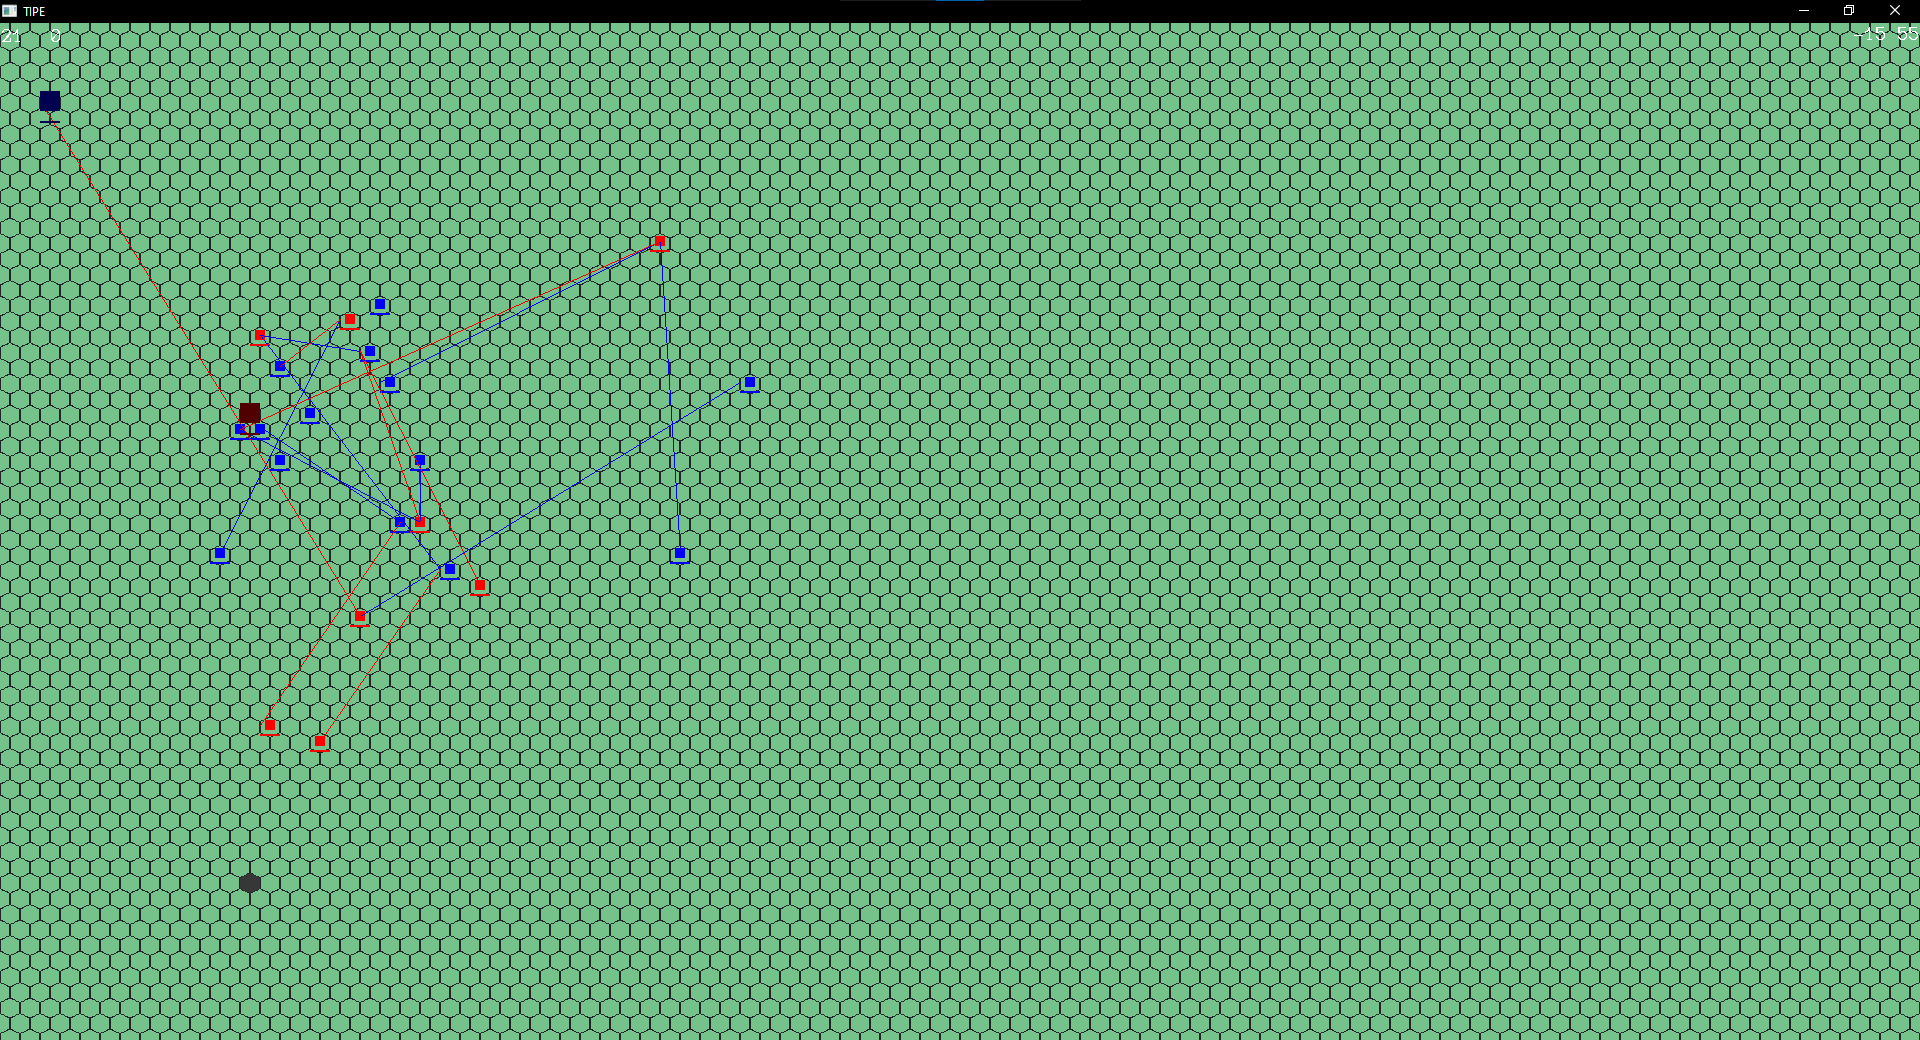
\includegraphics[width=\textwidth]{screen.png}
    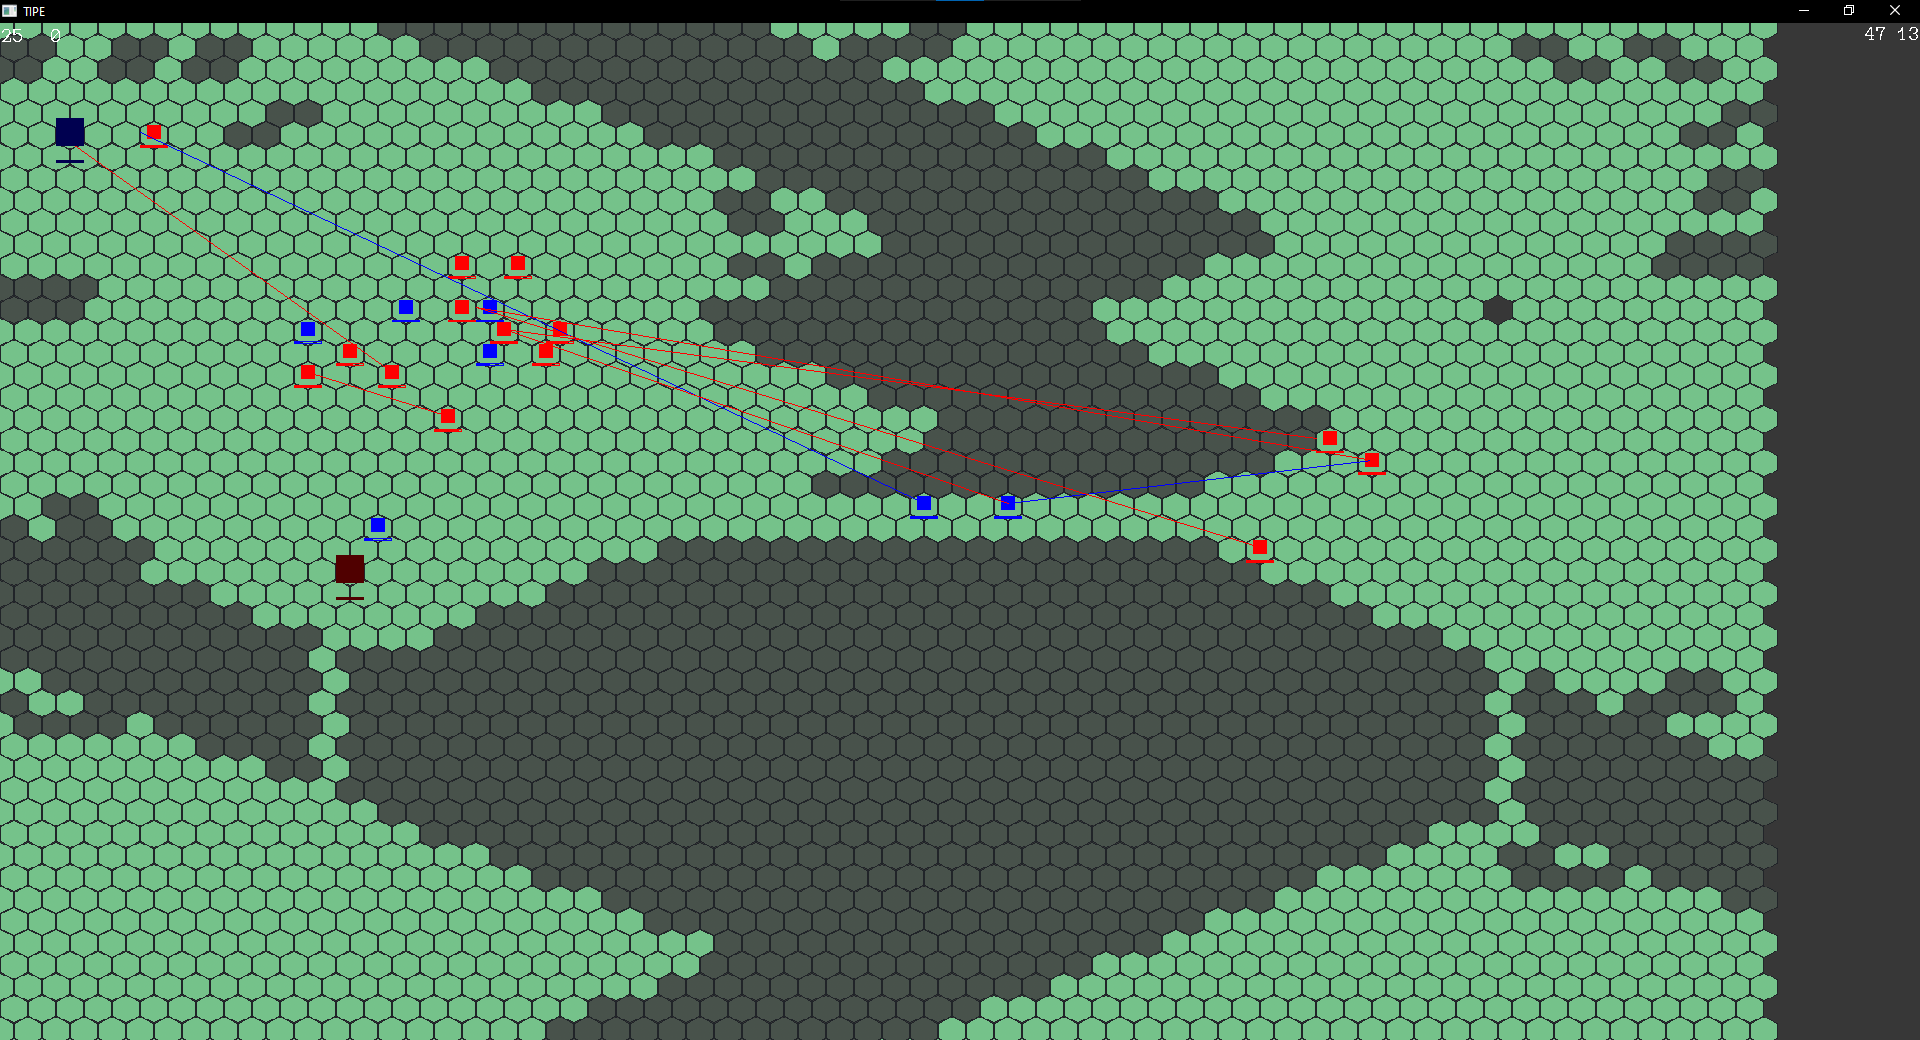
\includegraphics[width=\textwidth]{screen2.png}
    \caption{Captures d'écrans du programme}
\end{figure}
\vspace*{2em}
\begin{center}
\begin{tikzpicture}[%
    inner sep=3ex, semithick, ->, > = Latex,every node/.style={draw, rectangle, font=\sffamily}, align=center]
    \node(API) at (5,0) {API\\(interface de programmation)};
    \node(1) at (-3,0) {Joueur};
    \begin{scope}[transform canvas={yshift=.7em}]
        \draw(API) -- node[inner sep=1ex, above, draw=none]{Carte, unitées,\\actions possibles} (1);
    \end{scope}
    \begin{scope}[transform canvas={yshift=-.7em}]
        \draw(1) -- node[inner sep=1ex, below, draw=none]{Actions choisies} (API);
    \end{scope}

\end{tikzpicture}
\end{center}

\newpage
On définit trois objets:
\begin{description}
    \item[unité] $u = (p, hp, t_a, t_m, type)$
    \item[nourriture] $f = (p)$
    \item[base] $b = (p, hp)$
\end{description}

Chaque joueur contrôle des unités qu'il peut bouger et qui peuvent effectuer 4
actions :
\begin{itemize}
    \item Bouger l'unité $a$ à la position $p$
    \item Attaquer l'unité $b$ avec l'unité $a$
    \item Ramasser la nourriture $f$ avec l'unité $a$
    \item Attendre $t$ secondes
\end{itemize}

\section*{Joueur aléatoire}
\begin{tikzpicture}
    \begin{axis} [
        title={Joueurs aléatoires},
        ybar,
        bar width = 10mm,
        ymin = 0,
        ymax = 800,
        enlarge x limits=0.5,
        xtick = data,
        symbolic x coords={joueur 1, égalité, joueur 2},
    ]
     
    \addplot coordinates {({joueur 1},359) ({égalité},4) ({joueur 2},637)};
     
    \end{axis}
\end{tikzpicture}

\section*{Modèle simple de joueur avec stratégie groupée}
\begin{center}
\begin{tikzpicture}[%
    ->, > = Latex,every node/.style={draw, rectangle, font=\sffamily}, align=center]
    \node (Squad) at (-3,-3) {Squads};
    \node (Squad2) at (-3.1,-3.1) [behind path, fill=white]{Squads};
    \node (Squad3) at (-3.2,-3.2) [behind path, fill=white] {Squads};
    \node (Army) at (-2,-1.5) {Manager des\\armées};
    \node (Worker) at (3,-1.5) {Manager des\\travailleurs};

    \draw [ <->] (Army) -- (Worker);
    \draw [ -> ] (Army) -- (Squad);
    \node[minimum width = 20em, minimum height = 2em, thick] (API) at (0, -5){API};
    
    \begin{scope}[transform canvas={xshift=-1.5em}]
    \draw[semithick]    (API.north -| Army.south east) edge (Army.south east)
                        (API.north -| Worker)  to  (Worker);
    \end{scope}
    \node[draw, thick, inner sep=3ex, yshift=-1ex, fit=(Squad3) (Worker) (Army) (Squad)] (stratBox) {};
    \node[fill=white, inner xsep=1ex] at (stratBox.north) {Joueur};

    \draw[semithick, ->]    (Squad3.south) -- (Squad3.south |- API.north);;
\end{tikzpicture}
\end{center}

\section*{MaasCraft}
\begin{center}
\begin{tikzpicture}[%
    ->, > = Latex,every node/.style={draw, rectangle, font=\sffamily}, align=center]
    \node (Map) at (-5,0) {Analyseur de carte};
    \node (Units) at (-5,-0.9) {Analyseur d'unitées};
    \node (Strategy) at (1.5,0) {Manager des strategies};
    \node (Squad) at (0,-3) {Squads};
    \node (Squad2) at (0.1,-3.1) [behind path, fill=white]{Squads};
    \node (Squad3) at (0.2,-3.2) [behind path, fill=white] {Squads};
    \node (Army) at (0,-1.5) {Manager des\\armées};
    \node (Worker) at (3,-1.5) {Manager des\\travailleurs};

    \node[draw, thick, inner sep=3ex, yshift=-1ex, fit=(Strategy) (Worker) (Army) (Squad)] (stratBox) {};
    \node[fill=white, inner xsep=1ex] at (stratBox.north) {Décisions};

    \path let
    \p1 = (stratBox.north west),
    \p2 = (stratBox.south west),
    \n1 = {\y1-\y2} %\yN is y-coordinate of \pN
    in node[draw, thick, minimum height = \n1, inner sep=3ex, yshift=-\n1/2+3.9ex, fit=(Map)] (infoBox) {};
    \node[fill=white, inner xsep=1ex] at (infoBox.north) {Informations};

    \draw [ <-> , semithick] (infoBox.east) -- (stratBox.west);
    \draw [ <->] (Army) -- (Worker);
    \draw [ -> ] (Army) -- (Squad);
    \draw   (Strategy.south -| Army) edge (Army)
            (Strategy.south -| Worker)  to  (Worker);
    \path let
    \p1 = (infoBox.north west),
    \p2 = (stratBox.south west),
    \n1 = {-\x2-\x1}
    in node[minimum width = \n1, minimum height = 2em, thick] (API) at (\y1-5em, -5){API};
    \draw[semithick]    (API.north -| infoBox) edge (infoBox)
                        (API.north -| stratBox)  to  (stratBox);

    \draw[semithick, ->]    (Squad3.south) -- (Squad3.south |- API.north);;
\end{tikzpicture}
\end{center}
\begin{figure}[h]
    \centering
    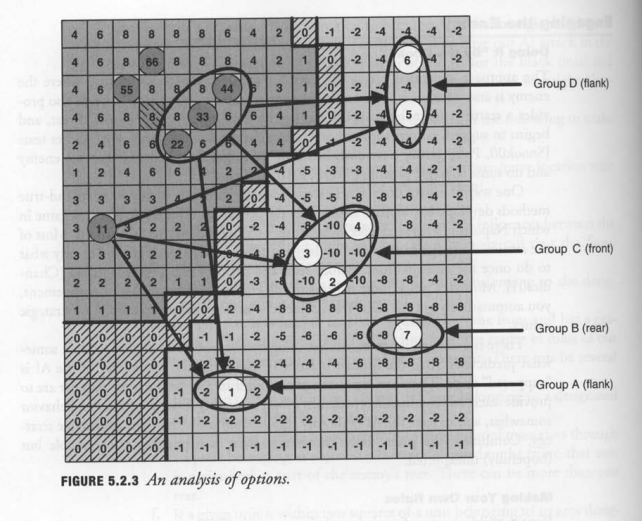
\includegraphics[width=\textwidth]{screen4.png}
    \caption{Analyse des positions}
\end{figure}
\begin{figure}[h]
    \centering
    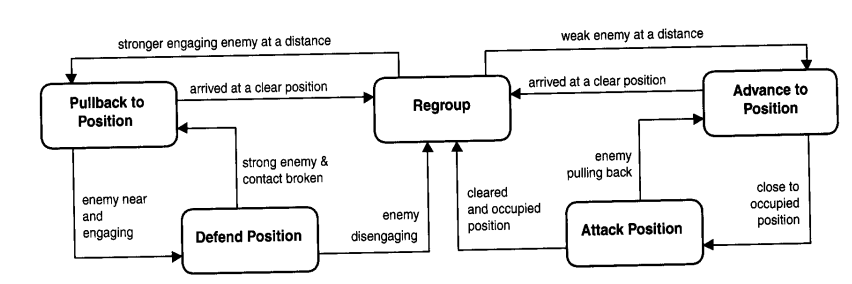
\includegraphics[width=\textwidth]{screen3.png}
    \caption{Machine à états finis}
\end{figure}


\end{document}
